\documentclass[UTF8]{ctexart}

\usepackage{geometry} 
\usepackage{setspace}
\usepackage{graphicx}
\usepackage{fancyhdr}

\geometry{left=30mm,right=30mm,top=25mm,bottom=25mm}
\setlength{\baselineskip}{30pt}

\title{\vspace{-1.5cm}第一部分需求文档\vspace{-2em}}
\pagestyle{fancy}
\fancyhf{} 
\rfoot{\thepage} 
\date{}

\begin{document}
\maketitle
\section{背景信息}
本部分基于饿了么仿真开发一个使用命令行的餐饮外卖平台管理系统,其中包括后台管理员和商家两个角色。

管理员可以管理商家信息,商家可以管理自己的商家信息和所属的食品。

\section{功能需求}

\subsection{后台管理员系统功能}

\begin{itemize}
    \item \textbf{登录系统}:管理员通过提供用户名和密码登录系统。
    \item \textbf{退出系统}:管理员可以退出系统。
    \item \textbf{查看商家列表}:管理员可以查看所有商家的列表信息,包括商家编号、商家名称、商家地址、商家介绍、起送费、配送费。
    \item \textbf{搜索商家}:管理员可以根据商家名称或地址关键词搜索商家。
    \item \textbf{新建商家}:管理员可以新建商家。新建商家时,管理员仅需提供商家名称,商家编号由数据库自动生成,商家地址、商家介绍、起送费、配送费等信息由商家后续自行填写。若创建成功,管理员会获得新建商家的编号。
    \item \textbf{商家删除}:管理员可以删除商家。删除商家时,管理员可通过列出的商家列表选择商家编号,并在确认删除后删除商家。
\end{itemize}

\subsection{商家管理系统功能}

\begin{itemize}
    \item \textbf{登录系统}:商家通过提供商家编号和密码登录系统。
    \item \textbf{退出系统}:商家可以退出系统。
    \item \textbf{查看商家信息}:商家可以查看自己的商家信息,包括商家编号、商家名称、商家地址、商家介绍、起送费、配送费。
    \item \textbf{修改商家信息}:商家可以修改自己的商家信息,包括商家名称、商家地址、商家介绍、起送费、配送费。
    \item \textbf{更新密码}:商家可以通过提供旧密码更新自己的登录密码。
    \item \textbf{管理所属食品}:商家可以对自己售卖的食品进行管理。
    \begin{itemize}
        \item \textbf{查看食品列表}:商家可以查看属于自己的食品列表信息,包括食品编号、食品名称、食品介绍、食品价格。
        \item \textbf{新建食品}:商家可以添加新的食品信息,需要提供新增食品的名称、介绍、价格。
        \item \textbf{修改食品}:商家可以修改已有的食品信息,包括食品名称、食品介绍、食品价格。
        \item \textbf{删除食品}:商家可以删除食品信息。删除食品时,商家可通过列出的食品列表选择商食品编号,并在确认删除后删除食品。
    \end{itemize}
\end{itemize}

\section{用户角色}
系统中有两种用户角色:后台管理员和商家。

\section{用户界面}
系统使用命令行界面,管理员登录后显示管理员管理菜单,包含查看商家列表、搜索商家、新建商家、删除商家、退出系统的选项。

商家登录后显示商家管理菜单(一级菜单),包含查看商家信息、修改商家信息、更新密码、所属食品管理、退出系统的选项。

商家选择所属食品管理选项后,进入食品管理菜单(二级菜单),包括查看食品列表、新增食品、修改食品、删除食品、返回一级菜单的选项。

\section{数据管理}
本系统使用了Mysql数据库来存储这些信息,以进行管理员和商家登录验证和商家和食品数据的增删查改操作。


\begin{figure}[ht]
    \centering
    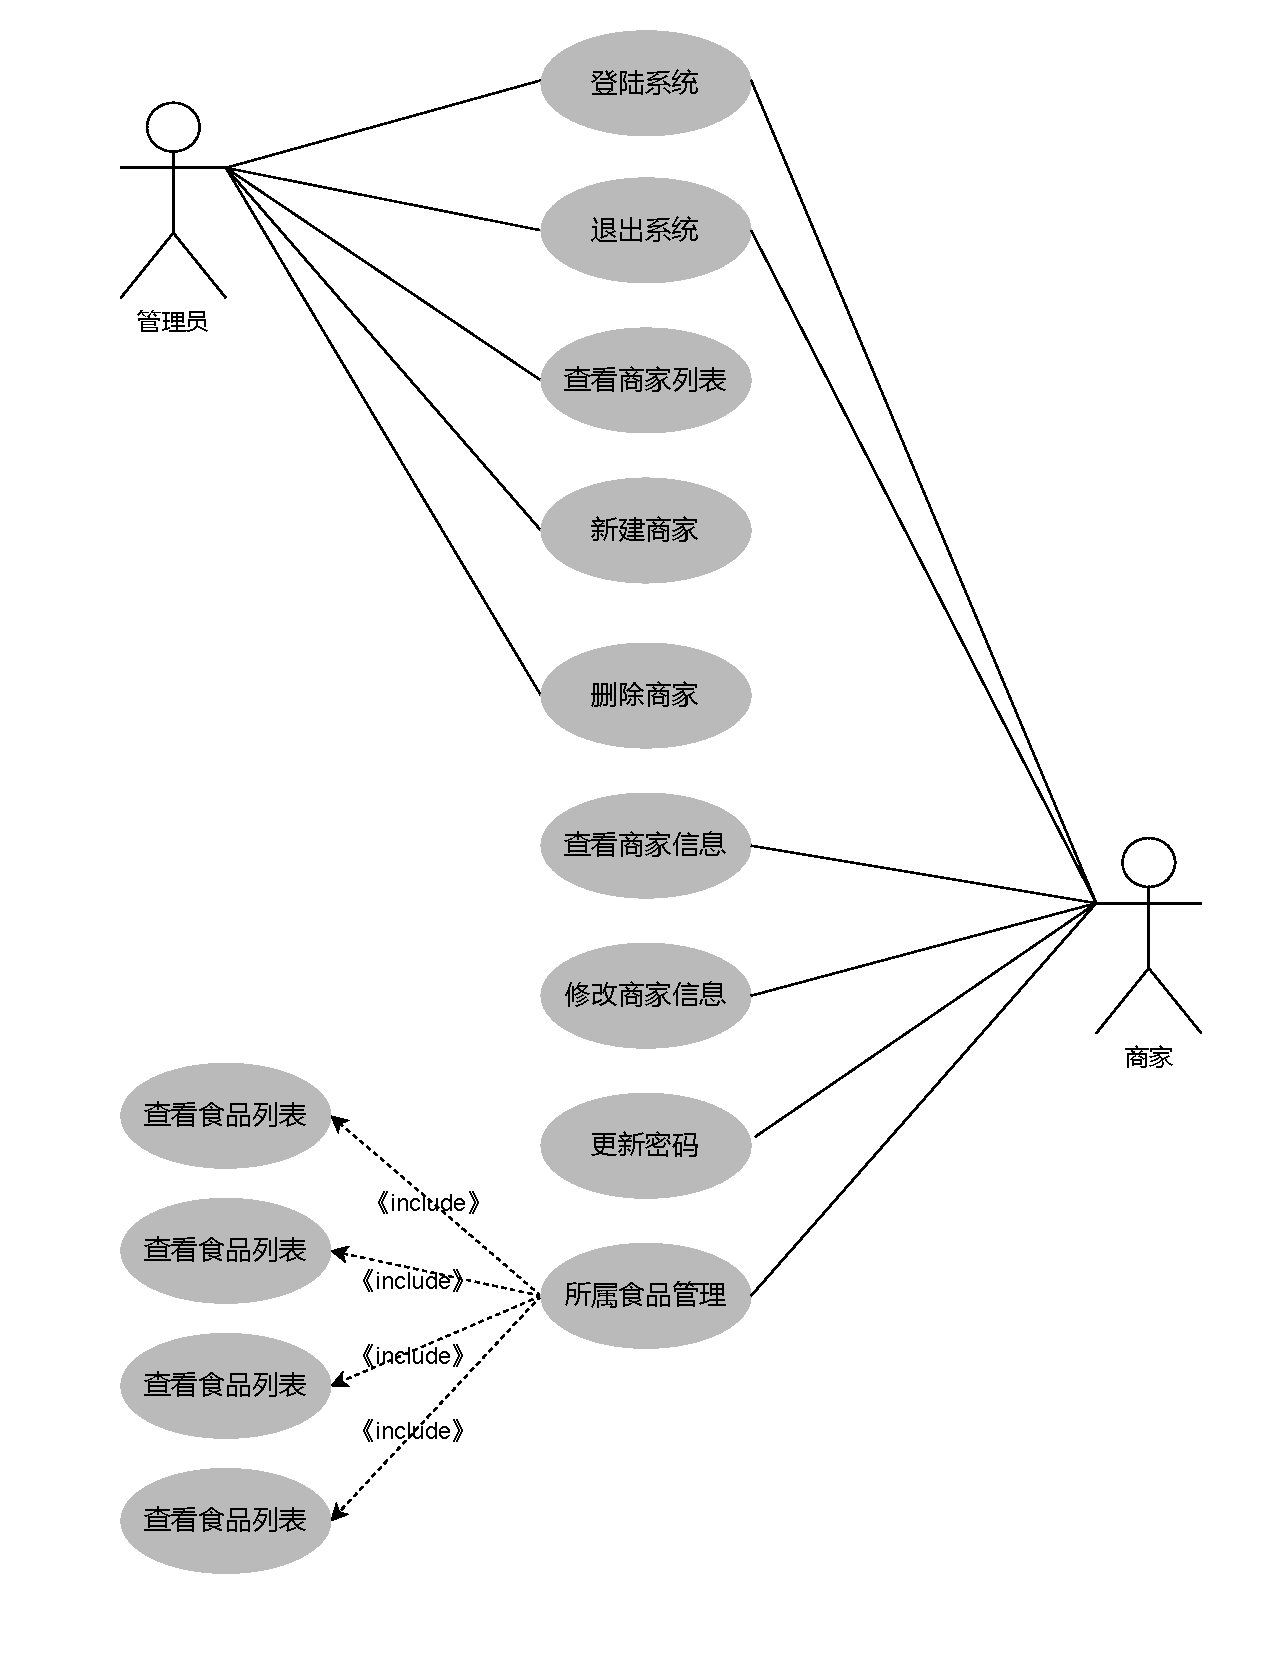
\includegraphics[width=\textwidth]{use_case_diagram.pdf}
    \caption{用例图示例}
    \label{fig:use-case-diagram}
  \end{figure}

\end{document}
